\chapter{Concept}

In this chapter the concept of transferring \gls{AutoML} concepts to clustering will be described.
For this, it will first be explained how meta-learning and the hyperparameter optimization methods were used to optimize the parameters of a clustering algorithm.
After this, the changes that had to made to the concept to also tackle the problem of algorithm selection  will be explained.


\section{Hyperparameter Optimization for Clustering}

\begin{itemize}
    \item First applied concepts on KMeans.
    \item Goal is to predict the number of clusters.
    \item For this, analyze which hyperparameter optimization methods are suitable.
    \item Also analyze which metrics are suitable for the different methods.
    \item So use internal/external metrics for the optimizers.
    \item Although external cannot be applied for new unseen datasets since they do not have class labels.
    \item But meta-learning can be used to warmstart optimizers.
    \item Warmstart means that the optimizers do not start with random models but with models that are suggestes by meta-learning model.
    \item For this, offline phase necessary.
    \item Assuming in the offline phase the number of clusters is known, it is also possible to use external metrics.
    \item Basic architecture shown in \cref{fig:concept_arch}.
    \begin{figure}
        \centering
        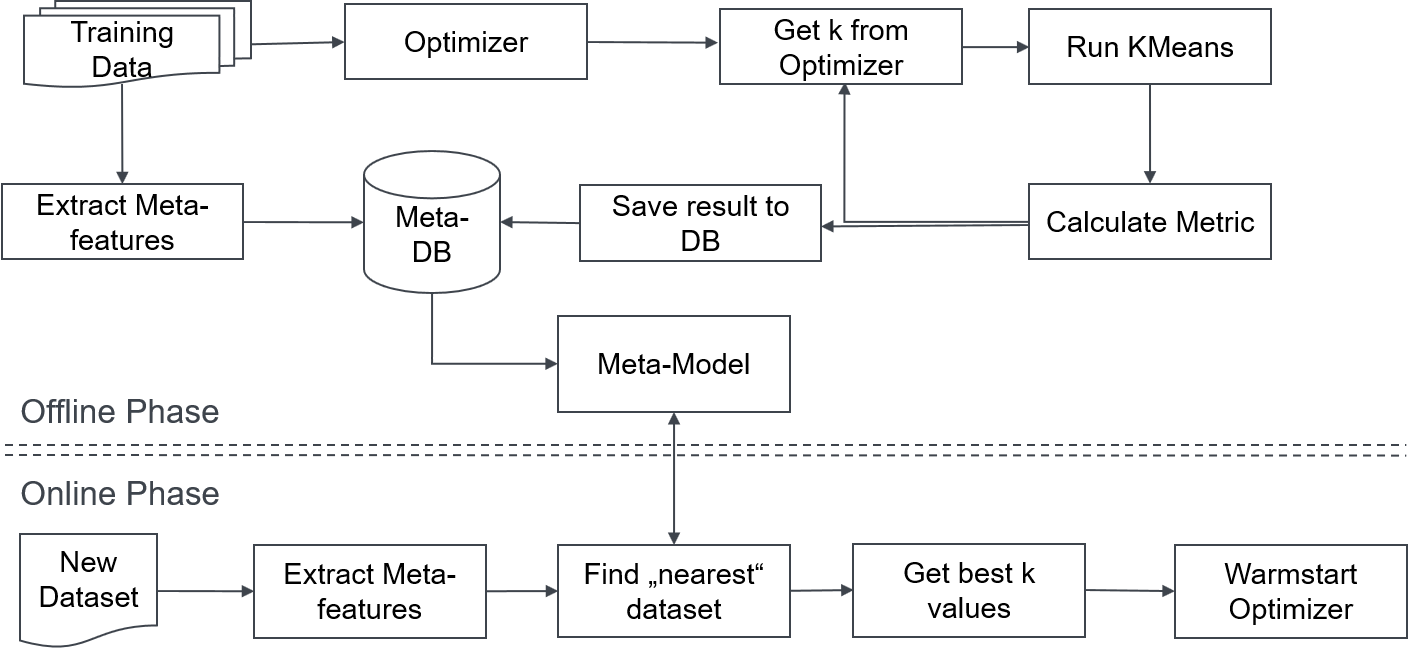
\includegraphics[width=\textwidth]{graphics/concept_architecture.png}
        \caption{General architecture of the concept divided in Online and Offline phase.}
        \label{fig:concept_arch}
    \end{figure}
    \item Offline phase: Train ``meta-model''
    \item Use optimizer to get configuration. Run KMeans on them and evaluate resulting according to metric.
    \item Then save result to Meta-DB.
    \item Also save the evaluation of the dataset together with the \textit{meta-features}.
    \item Meta-DB builds the meta-model.
    \item For the meta-model a k-NN classifier with $k=1$ is used.
    \item If new dataset has to be clustered in online phase, then extract meta-features (same as in offline phase). 
    \item Then find the ``nearest'' dataset.
    This is basically where 1-NN is used to find the nearest dataset based on the $L1$ distance.
    \item Input is meta-features of the new dataset and these are used to build the 1-NN and find the nearest dataset.
    \item From the nearest dataset it is looked up for which configurations the lowest k deviation was measured in the offline phase.
    \item This configurations are then used to \textit{warmstart} the optimizer, which means the optimizer first evaluates this configurations.
    
    
    
    
\end{itemize}
 
 
\section{Algorithm Selection for Clustering}

\begin{itemize}
    \item Basically same as for Hyperparameter Selection.
    \item Instead of only using parameters of that one algorithm, the optimizer gets one additional parameter.
    \item Additional parameter is name of algorithm.
    \item So the optimizer predicts the name of the algorithm and the hyperparameters like done in \cite{ThorntonAuto-WEKA:Algorithms}.
    \item Limited to partitional clustering algorithms.
    \item Basically Bayes would also be applicable to other clustering algorithms, but for multi-arm bandit based methods the budget has to be defined somehow.
    To get a meaningful metric result one needs labels for all data points after each iteration if the budget is the number of iterations or even for time budget.
    This holds partitional clustering algorithms but not necessarily for other kinds of clustering algorithms.
    \item The architecture shown in \cref{fig:concept_arch} changes in that way that the optimizer does not only gives the k value that should be executed next, but also the algorithm.
    \item New architecture can be seen in \cref{fig:archAlgoSelection}.
    \begin{figure}
        \centering
        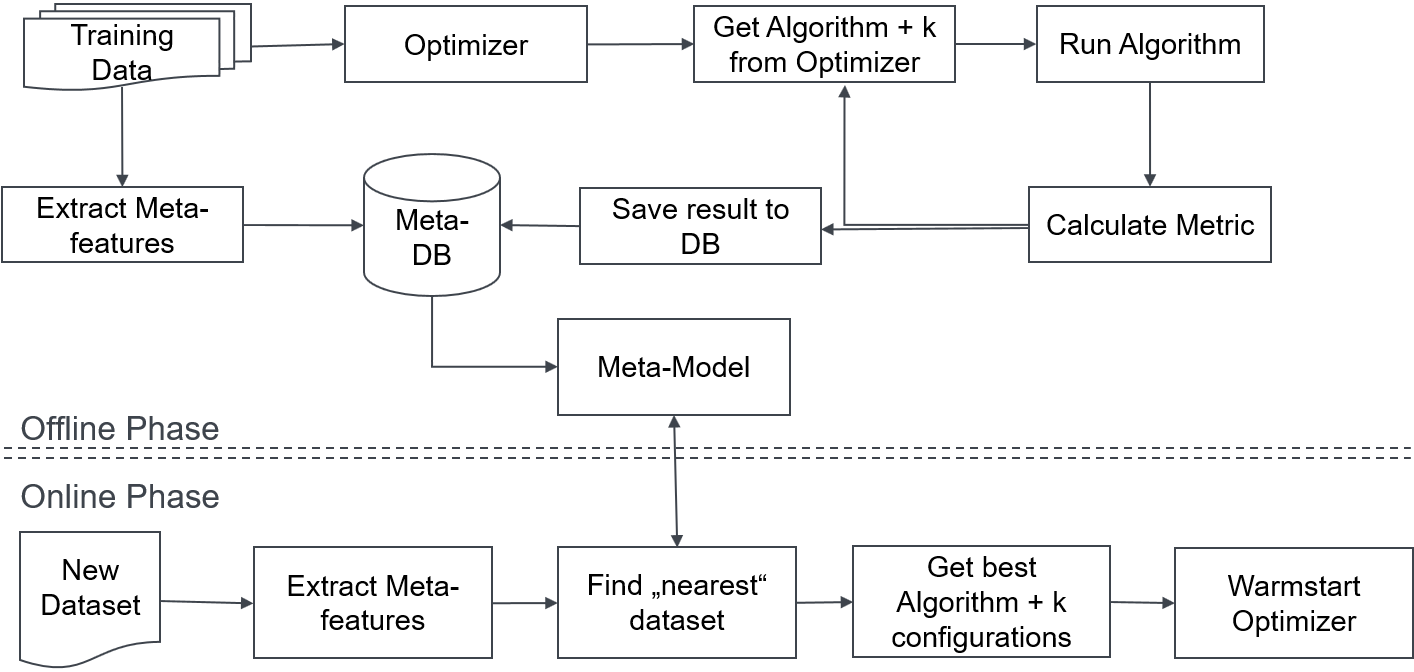
\includegraphics[width=\textwidth]{main/concept_architecture_algo_selection.png}
        \caption{General architecture of the concept to also include the algorithm selection.}
        \label{fig:archAlgoSelection}
    \end{figure}
    
\end{itemize}